\documentclass[12pt]{article}
\usepackage[utf8]{inputenc}
\usepackage[english]{babel}
\usepackage[a4paper,margin=1in]{geometry}
\usepackage[singlespacing]{setspace}
\usepackage{hyperref}
\usepackage{graphicx}
\graphicspath{{./figures/}{./images/}}
\usepackage{amsmath,amssymb,amsfonts,amsthm}
\usepackage{enumitem}
\usepackage{fix-cm}
\usepackage[autostyle, english=american]{csquotes}
\MakeOuterQuote{"}

% for the bibliography, requires that biber be installed
\usepackage[backend=biber]{biblatex}
% specify the bib file to build from
\addbibresource{temp.bib}

%%%%%%%%%%%%%%%%%%%%%%%%%%%%%%%%%%%%%%%%%
%          Front Matter Configs         %
%%%%%%%%%%%%%%%%%%%%%%%%%%%%%%%%%%%%%%%%%

%%%%%%%%% TOC formatting %%%%%%%%%
\setcounter{tocdepth}{2}
\usepackage{tocloft}
\addto\captionsenglish{
	\renewcommand{\contentsname}{Table of Contents}
	\renewcommand\listfigurename{\vspace{-15mm}}
	\renewcommand{\listtablename}{\vspace{-10mm}}
}
\renewcommand{\cftsecleader}{\cftdotfill{\cftdotsep}}
\renewcommand\cfttoctitlefont{\hfill\Large\bfseries}
\renewcommand\cftaftertoctitle{\hfill\mbox{}}
\renewcommand\cftloftitlefont{\hfill\Large\bfseries}
\renewcommand\cftafterloftitle{\hfill\mbox{}}
\addtocontents{lof}{\linespread{2}\selectfont}
\addtocontents{lot}{\linespread{2}\selectfont}
% removes line numbering for TOC
\def\numberline#1{}
\makeatletter
\newcommand \Dotfill {\leavevmode \cleaders \hb@xt@ .8em{\hss .\hss }\hfill \kern \z@}
\makeatother
%%%%%%%%%%%%%%%%%%%%%%%%%%%%%%%%%%

% For combined figures and tables list
%\def\table{\def\figurename{Table}\figure}
%\let\endtable\endfigure 
\usepackage[font=small,format=plain,labelfont=bf,up,textfont=normal,up,justification=justified,singlelinecheck=false]{caption}

% Section formatting
\usepackage{titlesec}
\newcommand{\sectionbreak}{\clearpage}
%uncomment to print section number
%\titleformat{\section}[block]{\normalfont\fontsize{14}{15}\bfseries\filcenter}{\thesection}{1em}{}
\titleformat{\section}[block]{\normalfont\fontsize{14}{15}\bfseries\filcenter}{}{1em}{}
\titleformat{\subsection}[block]{\normalfont\fontsize{12}{15}\bfseries}{}{0px}{}
\titleformat{\subsubsection}[runin]{\normalfont\fontsize{12}{15}\bfseries}{}{0px}{}

% Document paragraph and indent spacing
\setlength\parindent{0pt}
\setlength\parskip{1em}

%%%%%%%%%%%%%%%%%%%%%%%%%%%%%%%%%%%%%%%%%
%       End of Front Matter Configs     %
%%%%%%%%%%%%%%%%%%%%%%%%%%%%%%%%%%%%%%%%%

%used for dummy text to test formatting
\usepackage{blindtext}

%%%%%%%%%%%%%%%%%%%%%%%%%%%%%%%%%%%%%%%%%
%        Setting and Variables          %
%%%%%%%%%%%%%%%%%%%%%%%%%%%%%%%%%%%%%%%%%
\date{}
\newcommand{\ProposalTitle}{Example Latex Layout for ENGR 3080}
\newcommand{\preparee}{Individual's Name}
\newcommand{\prepareeTitle}{Title}
\newcommand{\company}{Company Name}
\newcommand{\address}{Address line 1\\Address line 2}
% If you have a title page figure
% this label will show up in the list of tables
\newcommand{\titlepagefigure}{Title Page Figure}
\newif\iftitlefigure
% set this boolean true or false
\titlefiguretrue
%\titlefigurefalse

\begin{document}

%%%%%%%%%%%%%%%%%%%%%%%%%%%%%%%%%%%%%%%%%
%             Title Page                %
%%%%%%%%%%%%%%%%%%%%%%%%%%%%%%%%%%%%%%%%%
\hypersetup{pageanchor=false}
\begin{titlepage}
\centering
\linespread{1.7}
%{\fontsize{18pt}{24pt}\bfseries\ProposalTitle}\\
{\Large\bfseries\ProposalTitle}\\
\vspace{2cm}
\begin{large}
Prepared for:
\preparee, \prepareeTitle\\
\company\\
\address\\
\end{large}
\vspace{1.5cm}

%%%% Title Page Figure %%%% 
\iftitlefigure
	\begin{figure}[!ht]
		\centering
		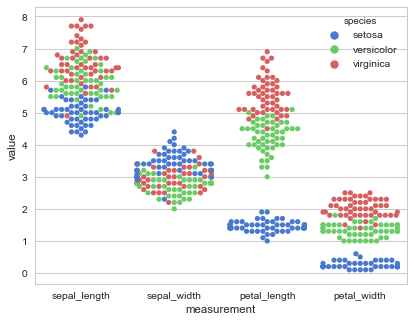
\includegraphics[width=0.6\linewidth]{swarmplot}
		\caption*{\centering\textbf{Swarm Plot Graph.} \textit{This is some caption text.}}
		\label{fig:titlepage}
	\end{figure}
	\stepcounter{figure}
\fi

\begin{large}
Prepared by:\\
Student Name, Title\\
Student Name, Title\\
Student Name, Title\\
\vspace{1cm}
\today\\
\end{large}


\vspace{1.5cm}
This is an example of what your topic overview might look like.  The purpose of proposal and the main topics covered are identified in this descriptive abstract.
\end{titlepage}
\hypersetup{pageanchor=true}
%%%%%%%%%%%%%%%%%%%%%%%%%%%%%%%%%%%%%%%%%
%           End of Title Page           %
%%%%%%%%%%%%%%%%%%%%%%%%%%%%%%%%%%%%%%%%%

\pagenumbering{roman}
\setcounter{page}{1}

\section{Executive Summary}
\blindtext

\clearpage
\tableofcontents
\clearpage

\addcontentsline{toc}{section}{List of Figures and Tables}
\begin{center}
{\fontsize{18pt}{24pt}\bfseries List of Figures and Tables}
\end{center}
%%%%% If you have a figure on the title page uncomment this line %%%%%
\iftitlefigure
	{\hspace{6mm}\fontsize{14pt}{15pt}\hyperref[fig:titlepage]{Figure \thefigure. \titlepagefigure} \Dotfill Title Page}
\fi

\listoffigures
\listoftables
\clearpage

\pagenumbering{arabic}
\setcounter{page}{1}

\section{Top Level Section}
\blindmathtrue
\blindtext

See my cool truth table (\ref{tab:truthy})

\begin{table} [h!]
\caption[Table \thetable. Truth Table]{ \textbf{A Truth Table.} } 
\begin{tabular} {c c c | c}
p & q & r & S\\ \hline
1 & 1 & 1 & 1\\
1 & 1 & 0 & 1\\
1 & 0 & 1 & 1\\
1 & 0 & 0 & 1\\
0 & 1 & 1 & 1\\
0 & 1 & 0 & 1\\
0 & 0 & 1 & 1\\
0 & 0 & 0 & 1\\
\end{tabular}
\label{tab:truthy}
\end{table}

\blindtext

And see my cool Cubehelix Graph (\ref{fig:cubehelix}).

\begin{figure}[!ht]
	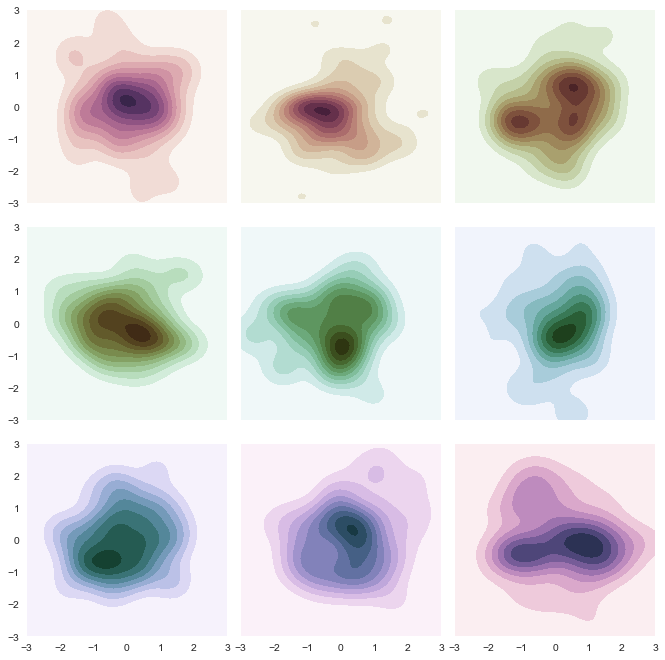
\includegraphics[width=0.4\linewidth]{cubehelixpalette}
	\caption[Figure \thefigure. Cubehelix Graph]{ \textbf{Cubehelix Graph.} \textit{This is some caption text.}}
	\label{fig:cubehelix}
\end{figure}

This is a citation\cite[chapter, p.~15]{greenwade93}.
And another citation\cite{goossens93}.

\begin{figure}[!ht]
	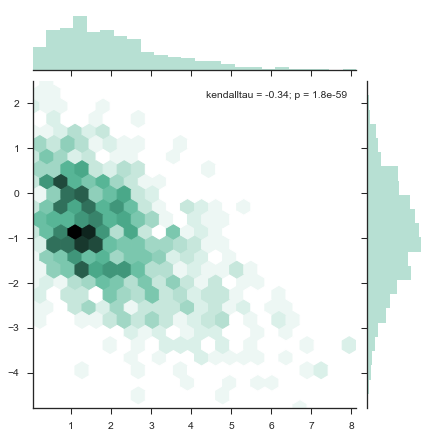
\includegraphics[width=0.4\linewidth]{hexbinmarginals}
	\caption[Figure \thefigure. Hexbin Marginal Graph]{ \textbf{Hexbin Graph.} }
	\label{fig:hexbin}
\end{figure}

Here is a crazy equation in \LaTeX
\begin{equation} \label{eq:crazy}
	\frac{\sin(2x + \pi)}{\cos(\int_0^\infty{\lambda_1 + \lambda_2})}
\end{equation}

See crazy equation (\ref{eq:crazy}).

\section{Level Section}
\blindtext
\blinditemize
\subsection{Second Level Heading}
\blindtext
\blindenumerate
\subsubsection{Third level inline.}
\blindtext
\section{Another Section}
\blindtext
\par
\blindtext
\subsection{Subsection}
\blindtext
\section{Another Section}
\blindtext
\par
\blindtext
\subsection{Subsection}
\blindtext

\section{Appendix A}
\blindtext
\blinditemize
\section{Appendix B}
\blindtext

\printbibliography

\end{document}
